% Appendix
\clearpage
\appendix

\setcounter{page}{1}
\setcounter{linenumber}{1}
% \setcounter{table}{6}
% \setcounter{equation}{9}

\section*{\LARGE Supplementary Material}
\label{supp}


\section{Supplementary Overview}
% This supplementary document provides comprehensive implementation details, extended evaluations, and interactive visual proofs to further validate the contributions of AirSplat. Specifically, Sec.~\ref{sec:supp_implementation_details} outlines our exact hyperparameter settings and training protocols. In Sec.~\ref{sec:supp_pose_geo_discrepancy}, we provide a detailed analysis of the pose-geometry discrepancy arising from the context-target training strategy. To fully assess this phenomenon and the effectiveness of our SCPA module, we strongly encourage readers to interact with the \href{./Supplementary_Viz/pose_geometry_discrepancy.html}{pose\_geometry\_discrepancy.html} file located in the \textit{\textbf{Supplementary\_Viz}} directory. This file features visual samples demonstrating the distinct spatial misalignment between the ground-truth (GT) and renderings produced without SCPA, explicitly accompanied by the precise geometric alignment achieved when our SCPA module is applied. Furthermore, Sec.~\ref{sec:supp_ablation_study} validates the generalizability of our framework with additional ablation studies on the DL3DV dataset~\cite{ling2024dl3dv}, while Sec.~\ref{sec:supp_geometry_estimation} benchmarks AirSplat's visual geometry estimation against prior NVS methods. We also analyze the computational trade-offs of SCPA's training overhead in Sec.~\ref{sec:supp_training_overhead} and discuss our framework's inherent limitations in Sec.~\ref{sec:supp_limitations}. Finally, Sec.~\ref{sec:supp_experimental_results} presents extended qualitative comparisons, supplemented by the \href{./Supplementary_Viz/supp_videos.html}{supp\_videos.html} file in the \textit{\textbf{Supplementary\_Viz}} which features side-by-side NVS video comparisons between the DepthAnything3 (DA3)~\cite{lin2025da3} baseline and AirSplat.

This supplementary document provides comprehensive implementation details, extended evaluations, and interactive visual proofs to further validate the contributions of AirSplat. Specifically, Sec.~\ref{sec:supp_implementation_details} outlines our exact hyperparameter settings and training protocols. In Sec.~\ref{sec:supp_pose_geo_discrepancy}, we provide a detailed analysis of the pose-geometry discrepancy arising from the context-target training strategy. Furthermore, Sec.~\ref{sec:supp_ablation_study} validates the generalizability of our framework with additional ablation studies on the DL3DV dataset~\cite{ling2024dl3dv}, while Sec.~\ref{sec:supp_geometry_estimation} benchmarks AirSplat's visual geometry estimation against prior NVS methods. We also analyze the computational trade-offs of SCPA's training overhead in Sec.~\ref{sec:supp_training_overhead} and discuss our framework's inherent limitations in Sec.~\ref{sec:supp_limitations}. Finally, Sec.~\ref{sec:supp_experimental_results} presents extended qualitative comparisons.

% Also, we strongly encourage readers to view the accompanying \href{./Supplementary_Viz/supp_videos.html}{supp\_videos.html} and \href{./Supplementary_Viz/pose_geometry_discrepancy.html}{pose\_geometry\_discrepancy.html} files, located in the \textit{\textbf{Supplementary\_Viz}} directory, to fully assess the visual quality of our framework.
% The \href{./Supplementary_Viz/supp_videos.html}{supp\_videos.html} file provides a direct NVS performance comparison between the baseline DepthAnything3 (DA3) \cite{lin2025da3} and AirSplat on high-resolution images.
% Additionally, the \href{./Supplementary_Viz/pose_geometry_discrepancy.html}{pose\_geometry\_discrepancy.html} file features visual samples demonstrating the distinct spatial misalignment between the ground-truth (GT) and renderings produced without SCPA, explicitly accompanied by the successful, precise geometric alignment achieved when our SCPA module is applied.



\section{Implementation Details}
\label{sec:supp_implementation_details}
We employ the AdamW optimizer \cite{loshchilov2017adamw} with a learning rate of $2 \times 10^{-6}$ and a weight decay of $0.01$. 
We use a OneCycleLR \cite{smith2019super} scheduler with a warm-up period of $2,000$ steps. In Rating-based Opacity Matching (ROM), we set the error decay rate $\gamma=5.0$ and the stability constant $\eta=10^{-7}$. 
The loss weights are empirically determined as $\lambda_\text{geo}=0.1$ and $\lambda_\text{opa}=1.0$, while $\lambda_{s}$ is set to 0.1 for the LPIPS term. 
The complete training process requires approximately 4.5 days utilizing four NVIDIA A100 (40GB) GPUs.
During evaluation, we assess NVS performance using image resolutions of $252 \times 448$ for the DL3DV dataset \cite{ling2024dl3dv} and $252 \times 252$ for the RE10K dataset \cite{zhou2018stereo}.

\noindent \textbf{Rating-based Opacity Matching.}
Fig.~\ref{fig:teacher_rating} further clarifies our strategy for partitioning the input sequence to compute the teacher's geometric ratings. Since we utilize a two-view feed-forward 3DGS model \cite{xu2025depthsplat} as the teacher model, the input sequence is divided into pairs of adjacent views. The geometric errors of the pixel-aligned primitives are then computed separately for each pair using Eq.~\ref{eq:teacher_error}.
Once computed, these pairwise ratings are aggregated across the sequence to map each primitive to its corresponding opacity penalty, rigorously enforcing local multi-view consistency before dynamically compressing the student's global opacity map.

\begin{figure*}[t]
    \centering
    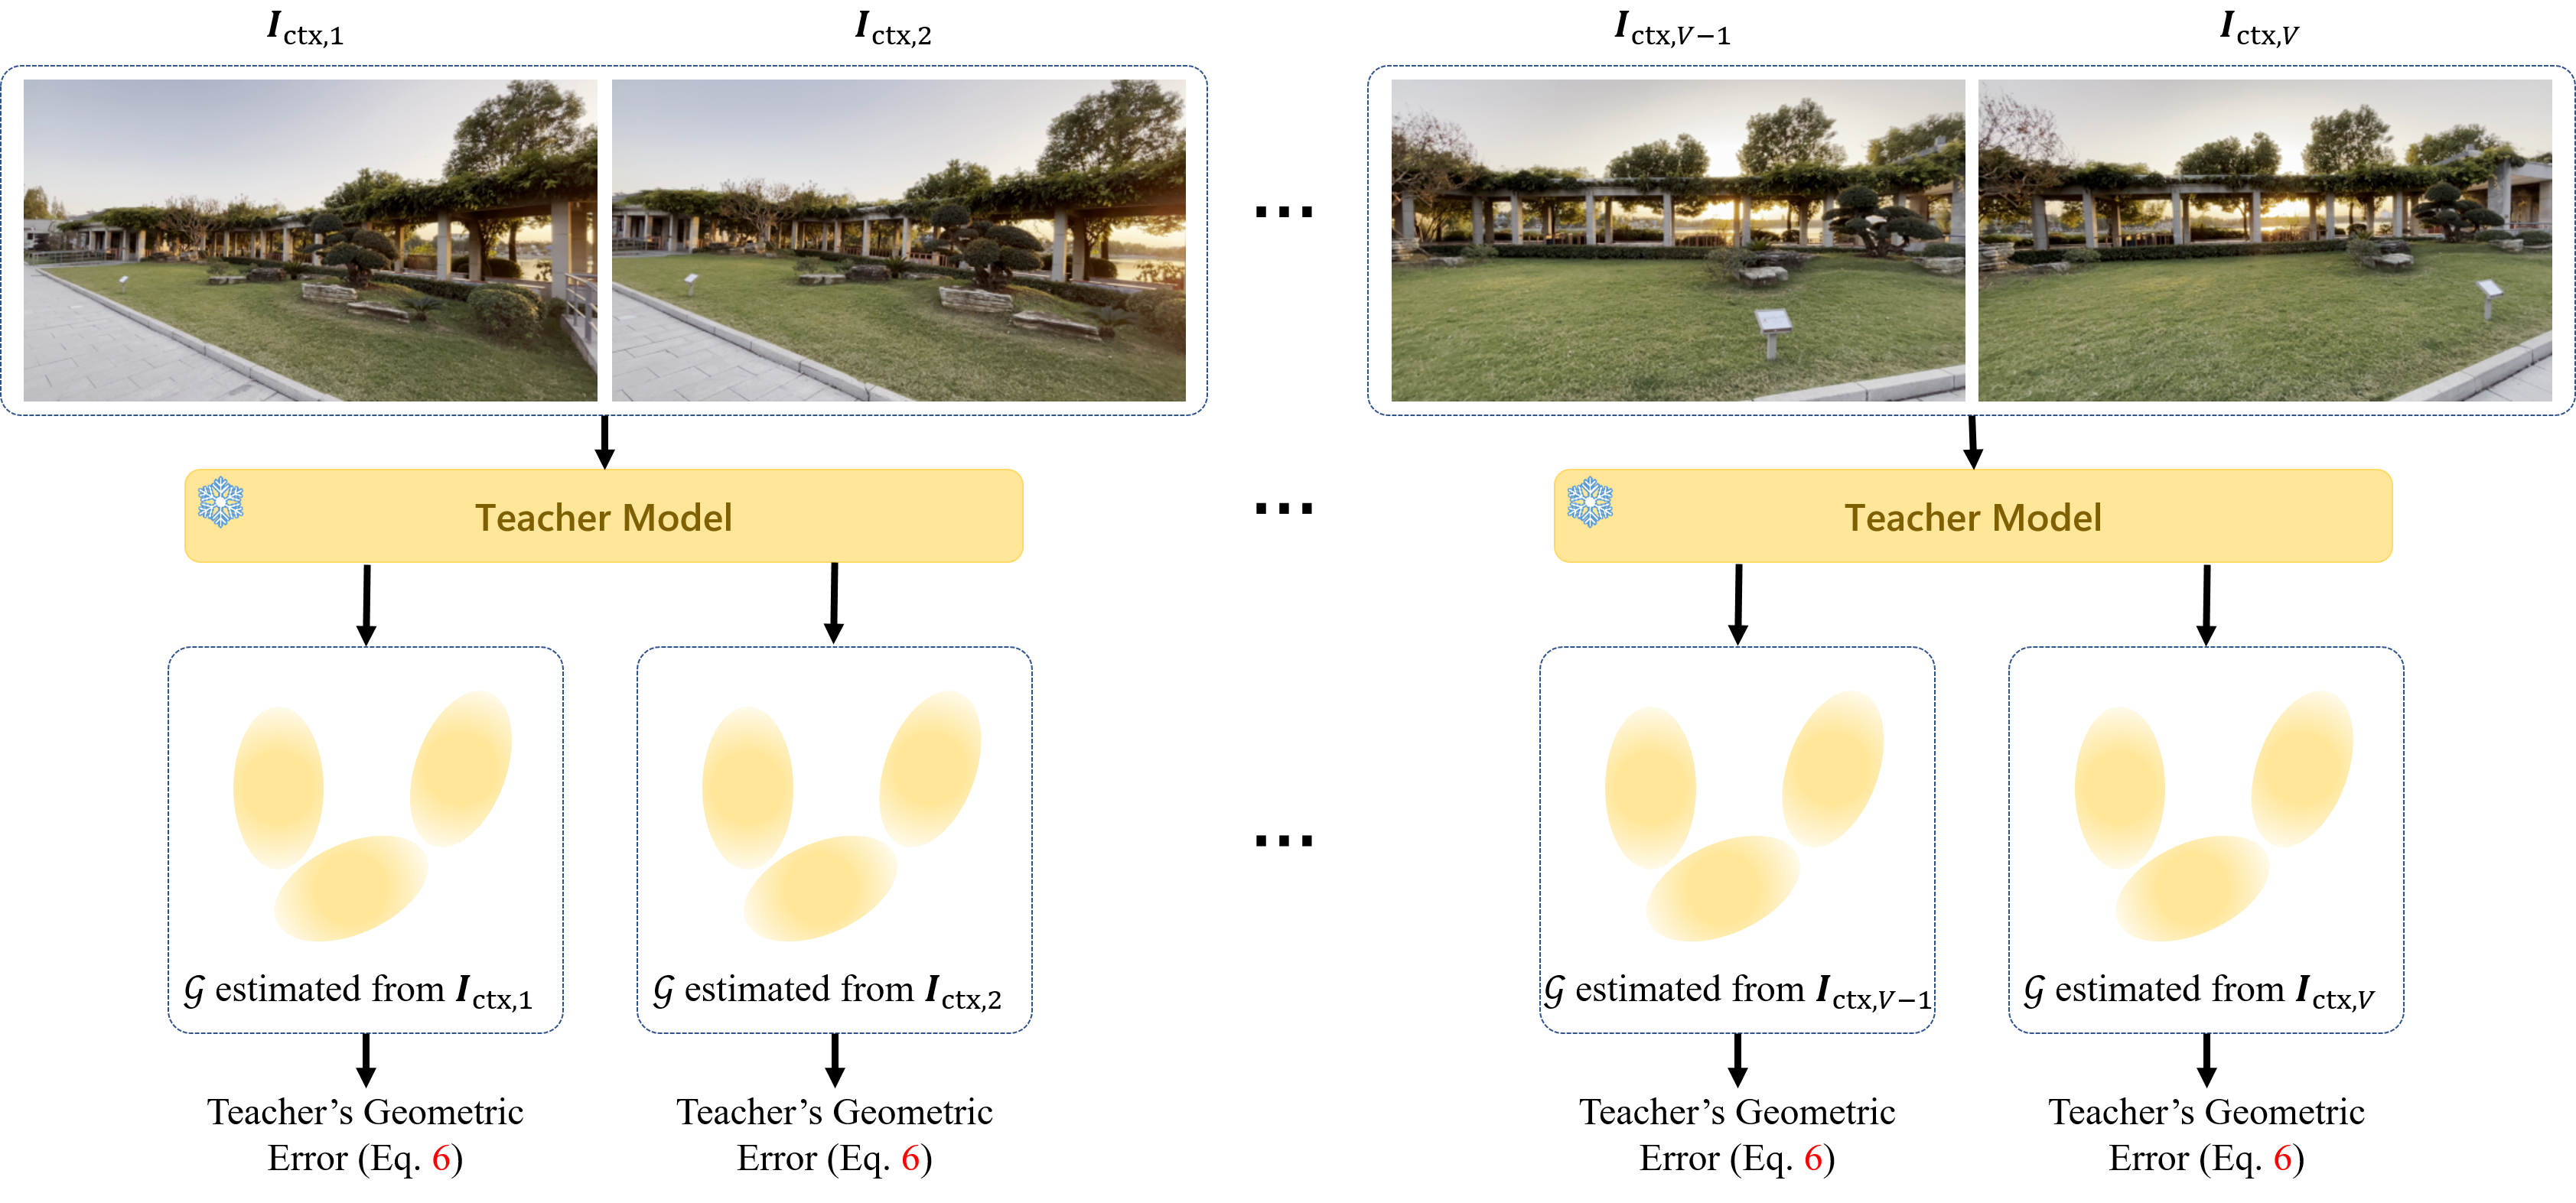
\includegraphics[width=0.9\linewidth]{figures/teacher_rating.png}
    \caption{Our strategy for partitioning input context sequences to compute the teacher's geometric errors.}
    \label{fig:teacher_rating}
\end{figure*}

% We adopt the Exponential Moving Average (EMA) \cite{tarvainen2017ema} weights updating strategy for stable training of the Gaussian head. 


\begin{figure*}[t]
    \centering
    \includegraphics[width=1\linewidth]{figures/supp_pose_geo_discrepancy.pdf}
    \caption{\textbf{Pose-Geometry Discrepancy.} To validate that this structural misalignment is not confined to a specific baseline, we visualize the consistent spatial drift across distinct models and diverse scenes: (a) DepthAnything3 \cite{lin2025da3} evaluated on the DL3DV dataset \cite{ling2024dl3dv}, and (b) SPFSplat \cite{huang2025no} on the RE10K dataset \cite{zhou2018stereo}.}
    \label{fig:supp_pose_geo_discrepancy}
\end{figure*}

\section{Pose-Geometry Discrepancy}
\label{sec:supp_pose_geo_discrepancy}

As discussed in Sec.~\ref{sec:scpa}, the asymmetric information flow within the context-target training strategy causes the predicted target poses to be misaligned with the predicted 3D Gaussian primitives. 
As shown in Fig.~\ref{fig:supp_pose_geo_discrepancy}, this pose-geometry discrepancy is a fundamental challenge, rather than an isolated issue confined to a specific baseline 3DVFM or dataset. 
To explicitly demonstrate this, we visualize the structural misalignment observed in DA3 \cite{lin2025da3} evaluated on the DL3DV dataset \cite{ling2024dl3dv}, alongside the discrepancy found in SPFSplat \cite{huang2025no} on the RE10K dataset \cite{zhou2018stereo}. 
In the figure, the first column shows the ground truth (GT) target images $\bm{I}_{\text{tgt}, t}$. 
The second column shows the aligned render $\hat{\bm{I}}^{\text{align}}_{\text{tgt}, t}$ utilizing our SCPA, achieving high spatial alignment with $\bm{I}_{\text{tgt}, t}$. 
From the third column to the last, we display the systematic and repeated drift that occurs when recursively mapping the synthesized geometry back to the pose manifold to compute the target pose $\hat{\bm{P}}^{(i)}_{\text{tgt}, t}$ and its corresponding render $\hat{\bm{I}}^{(i)}_{\text{tgt}, t}$ (as in Eq.~\ref{eq:recursive_pose}). Although the misalignment of each image in $\{\hat{\bm{I}}^{(i)}_{\text{tgt}, t}\}$ amplifies compared to $\bm{I}_{\text{tgt}, t}$, leading to a severe PSNR drop, it follows a consistent and predictable pattern. 
By leveraging this trajectory, SCPA effectively uses $\hat{\bm{P}}^{(1)}_{\text{tgt}, t}$ and $\hat{\bm{P}}^{(2)}_{\text{tgt}, t}$ to mathematically recover the aligned pose $\hat{\bm{P}}^{\text{align}}_{\text{tgt}, t}$. 
Ultimately, these consistent observations across different architectures and environments strongly validate the critical necessity of our SCPA module. 
Our SCPA successfully harnesses the robust supervisory signals of novel target views reconstruction from the context-target training strategy while strictly eliminating the detrimental gradients caused by misaligned photometric supervision.

% For more comprehensive visualization, please refer to the accompanying \href{./Supplementary_Viz/pose_geometry_discrepancy.html}{pose\_geometry\_discrepancy.html} file in the \textit{\textbf{Supplementary\_Viz}} folder.

\section{Ablation Study on DL3DV Dataset}
\label{sec:supp_ablation_study}

\begin{table*}[t]
\begin{center}
    \scriptsize
    \caption{Ablation analysis on DL3DV dataset \cite{ling2024dl3dv} under 12 input views.}
    \resizebox{0.8\linewidth}{!}{ 
        \setlength{\tabcolsep}{6pt}
\renewcommand{\arraystretch}{1.2}

\begin{tabular}{l | ccc}
\toprule
Methods & PSNR$\uparrow$ & SSIM$\uparrow$ & LPIPS$\downarrow$ \\
\midrule
Baseline  & 20.74 & 0.691 & 0.242 \\
Baseline + Context-only Training & 21.39 & 0.717 & 	0.233 \\
Baseline + Context-Target Training & 21.52 & 0.727 & 0.221 \\
Baseline + Context-Target w/ SPCA Training & 22.29 & 0.740 & 0.214 \\
Baseline + ROM & 22.11 & 0.731 & 0.218 \\
\textbf{Ours (Full)} & \textbf{22.50} & \textbf{0.747} & \textbf{0.207} \\
\bottomrule
\end{tabular}
    }
\label{table:supp_abl_dl3dv}
\end{center}
\end{table*}

To further validate the generalizability and robustness of our proposed modules across diverse and complex environments, we conduct an additional ablation study on the DL3DV dataset \cite{ling2024dl3dv}. 
Table~\ref{table:supp_abl_dl3dv} demonstrates that the performance trends strictly align with the findings presented in the main paper. 
The context-only training gains marginal improvements (reaching 21.39 dB PSNR) compared to the baseline.
While the context-target training strategy yields a slight enhancement over the context-only one (21.52 dB PSNR), it remains bottlenecked by spatial misalignment. 
Integrating our Self-Consistent Pose Alignment (SCPA) successfully mitigates this pose-geometry discrepancy, driving a substantial performance leap to 22.29 dB PSNR (+$0.77$ dB over the context-target baseline). 
Similarly, the independent integration of Rating-based Opacity Matching (ROM) effectively filters out structural inconsistencies, elevating the baseline to 22.11 dB. 
Finally, our full AirSplat framework synergizes both global pose alignment and local structural refinement to achieve the highest performance across all metrics (22.50 dB PSNR, 0.747 SSIM, and 0.207 LPIPS). 
These consistent results confirm that our framework effectively unlocks high-fidelity NVS while preserving foundational geometric priors, regardless of the dataset scale or complexity.


\section{Geometry Estimation Performance Comparison}
\label{sec:supp_geometry_estimation}
Our decision to fine-tune only the Gaussian prediction head of the 3D-VS-VFM (following the paradigm of DA3~\cite{lin2025da3}) is a deliberate design choice aimed at achieving a unified model for both robust visual geometry and high-fidelity NVS. 
To analyze the effect of fine-tuning entire 3DVFMs for NVS on visual geometry performance, we evaluate multi-view reconstruction metrics on the 7-Scenes~\cite{6619221} dataset, following $\pi^3$~\cite{wang2025pi3}. 
We compare baselines including AnySplat~\cite{jiang2025anysplat}, VGGT~\cite{wang2025vggt}, $\pi^3$~\cite{wang2025pi3}, DA3 \cite{lin2025da3}, and our AirSplat. As quantitatively demonstrated in Table~\ref{table:mv_recon}, even with training distillation, AnySplat leads to degradations of the backbone VGGT's zero-shot geometric priors. With our training strategy, AirSplat obtains improved NVS quality while maintaining the visual geometry estimation performance of DA3 \cite{lin2025da3}.

\begin{table*}[t]
\begin{center}
    \scriptsize
    \caption{Pose-free point map estimation on 7-Scenes~\cite{6619221} dataset.}
    \setlength{\tabcolsep}{7pt}
\begin{tabular}{ll cccccc}
\toprule
\multirow{2}{*}{\textbf{Method}} & \multirow{2}{*}{\textbf{View}} & \multicolumn{2}{c}{Acc. $\downarrow$} & \multicolumn{2}{c}{Comp. $\downarrow$} & \multicolumn{2}{c}{NC. $\uparrow$} \\
\cmidrule(lr){3-4} \cmidrule(lr){5-6} \cmidrule(lr){7-8}
& & Mean & Med. & Mean & Med. & Mean & Med. \\
\midrule
VGGT~\cite{wang2025vggt} & \multirow{4}{*}{\textit{sparse}} & \textbf{0.044} & \textbf{0.025} & \textbf{0.056} & \textbf{0.033} & 0.733 & 0.845 \\
AnySplat~\cite{jiang2025anysplat} & & 0.080 & 0.053 & 0.120 & 0.072 & 0.684 & 0.785 \\
$\pi^3$~\cite{wang2025pi3}& & 0.047 & 0.029 & 0.075 & 0.049 & 0.742 & 0.841 \\
DA3 \cite{lin2025da3}/AirSplat & & 0.049 & 0.034 & 0.065 & 0.046 & \textbf{0.757} & \textbf{0.866} \\
\midrule
VGGT~\cite{wang2025vggt} & \multirow{4}{*}{\textit{dense}} & 0.022 & 0.008 & 0.026 & 0.012 & 0.666 & 0.760 \\
AnySplat~\cite{jiang2025anysplat} & & 0.040 & 0.015 & 0.030 & 0.011 & 0.648 & 0.732 \\
$\pi^3$~\cite{wang2025pi3}& & \textbf{0.016} & \textbf{0.007} & \textbf{0.022} & 0.011 & \textbf{0.689} & 0.792 \\
DA3 \cite{lin2025da3}/AirSplat & & 0.018 & \textbf{0.007} & 0.023 & \textbf{0.009} & 0.688 & \textbf{0.795} \\
\bottomrule
\end{tabular}
\label{table:mv_recon}
\end{center}
\end{table*}

% However, our proposed optimization framework (incorporating both SCPA and ROM) is not strictly bound to the 3D-VS-VFM architecture. To demonstrate its plug-and-play generalizability across disparate pose-free NVS pipelines, we additionally integrate our training strategy into SPFSplat~\cite{huang2025no}, improving this baseline of the RE10K dataset NVS performance (as shown in Table~\ref{tab:your_table_label})




\section{Training Overhead}
\label{sec:supp_training_overhead}

\begin{table*}[t]
\begin{center}
    \scriptsize
    \caption{Training time analysis. We report the average time per training iteration. While our proposed modules (SCPA and ROM) introduce additional forward passes and teacher model evaluations, the overall training remains tractable.}
    \resizebox{0.6\linewidth}{!}{ 
        
\begin{tabular}{l | c c}
\toprule
Methods & Avg. Time (s) / Iter. &  \\
\midrule
Baseline + Context-Target & 2.35 & \\
Baseline + Context-Target w/ SCPA & 3.67 &  \\
Ours (Full Model) & 3.89 &  \\
\bottomrule
\end{tabular}
    }
\label{table:training_overhead}
\end{center}
\end{table*}

We analyze the computational training complexity introduced by our proposed modules. As detailed in Table~\ref{table:training_overhead}, the integration of SCPA and ROM increases the average time per training iteration by approximately 65\%. 
This expected overhead primarily stems from the supplementary forward passes required for pose correction and the teacher model evaluations for geometric rating. 
Crucially, this computational requirement is strictly confined to the training phase, imposing absolutely zero additional burden during feed-forward inference. The significant leap in state-of-the-art NVS quality and structural consistency fully justifies this trade-off of training efficiency.


\section{Limitations}
\label{sec:supp_limitations}
 A primary limitation of our current framework, common among deterministic feed-forward NVS models, is its strict reliance on observed input context views. Because AirSplat does not explicitly hallucinate unseen structures, severe occlusions or entirely uncaptured areas may manifest as structural voids in the rendered novel views. To resolve these deterministic blind spots, future directions of this framework could integrate generative video diffusion priors as a post-processing module, allowing for the temporally consistent inpainting of geometrically plausible content within these occlusions.

% While AirSplat significantly improves the novel view synthesis quality of 3D-VS-VFMs, it inherently inherits certain fundamental limitations from the frozen foundation models. Specifically, our framework may struggle to reconstruct scenes dominated by highly specular reflections, transparent objects (e.g., glass), or extreme textureless areas. In such scenarios, the pre-trained encoder of the foundation model may fail to extract robust initial geometric correspondences, which consequently bounds the effectiveness of our subsequent refinement modules. 



\begin{figure*}[t]
    \centering
    \includegraphics[width=\linewidth]{figures/qualitative_dl3dv_supp.pdf}
    \caption{Qualitative comparison of NVS performance on DL3DV dataset \cite{ling2024dl3dv}.}
    \label{fig:qualitative_dl3dv_supp}
\end{figure*}

\section{Additional Qualitative Comparison}
\label{sec:supp_experimental_results}


Fig.~\ref{fig:qualitative_dl3dv_supp} provides a qualitative comparison of novel view synthesis (NVS) performance under various input-view settings on the DL3DV dataset \cite{ling2024dl3dv}. 
Compared to recent baseline methods, including DepthSplat \cite{xu2025depthsplat}, AnySplat \cite{jiang2025anysplat}, and WorldMirror \cite{liu2025worldmirror}, AirSplat consistently synthesizes significantly sharper and higher-quality renderings. 
For instance, as highlighted in the third row, AirSplat accurately reconstructs challenging high-frequency details, such as the thin structure of the pole, which are distorted or entirely missed by prior approaches. 
Furthermore, the first and last rows demonstrate our model's superior capability in preserving sharp structural boundaries. 
Notably, while baseline methods like DepthSplat, AnySplat, and WorldMirror tend to accumulate severe floater artifacts and blurring as the number of input views increases, AirSplat maintains a clean, geometrically consistent reconstruction, validating the robustness of our framework across varying input densities. 

% Furthermore, we provide the \href{./Supplementary_Viz/supp_videos.html}{supp\_videos.html} file in the \textit{\textbf{Supplementary\_Viz}} folder which demonstrates a direct and interactive NVS performance comparison between the baseline DepthAnything3 (DA3) \cite{lin2025da3} and AirSplat.
